\begin{task}[
  title=Astronomy application,
  id=astro,
  lead=CDS,
  PM=18,
  wphases={0-48},
  partners={CDS}
]

  Context: The CDS \TODO{introduce CDS} plays a unique and essential role in astronomy by adding
  value to published and reference data. CDS runs astronomical services that
  provide data for the world-wide astronomy research community. Its three main
  services (SIMBAD, VizieR and Aladin) are heavily used with up to one million
  queries per day.  These services be accessed through web interfaces, mainly
  for human interaction, as well as through programmatic interfaces, including
  the standardized protocols defined by the International Virtual Observatory
  Alliance.

  We will develop a Jupyter-based framework to efficiently access, explore,
  visualize and analyze reference data that is available through CDS services.
  We will provide scientific users with a set of customizable Jupyter notebooks
  for visualization and analysis tasks, providing a new level of
  interoperability with python libraries and notebooks as is highly demanded
  by the astronomy research community.

  The focus is on the two following user stories:
    \begin{compactitem}
        \item analysis of catalogue data results, up to billions of rows.
              Tabular data is the typical output of SIMBAD and VizieR data.
        \item modular dashboard-like interface providing a top level
              interactive view of the available data for a given astronomical
              object and enabling loading and analysis of those data.
    \end{compactitem}


  This task will rely on existing Python libraries to access CDS data
  (\textit{astroquery.[cds/simbad/vizier/xmatch]}) and to visualize them
  (\textit{GLUE, ipyvolume}).
  We will also improve existing Jupyter widgets (\textit{ipyaladin},
  interactive sky atlas running in the notebook) and develop a new widget to
  offer a tree-like view of available data.

  We will also develop Python libraries to allow integration and usage in
  notebook of existing CDS infrastructure services, namely CDSLogin (which
  provides authentication) and CDS MyData (remote storage space for tabular
  data).
  This will allow the user to interact with one's personal storage space from
  the notebook. It will also allow for advanced customisation.

  Initially, the notebooks generated will run locally on user
  machines.
\TODO{This two stage approach (above and below) is good. Can we split
  this into two tasks, or link each to a different milestone, to make
  this more visible?}

  Later on, we will run them on European Binder Service developed in \WPref{eosc}.

  Access to the notebooks will be provided as a one-click action option from
  SIMBAD and VizieR results pages.
  Thus, providing with a one-click way of visualizing, filtering and analyzing
these potentially large tables will bridge the gap between access and analysis
of the data, with zero installation for the user.

  These new developments will be an awaited and welcome addition to existing
  toolset. In fact, Python for Astronomy software ecosystem has known a constant
    steady growth in the latest years, as shown in figure~\ref{fig:python-astro-citations}.

  \begin{figure}[ht]\centering
  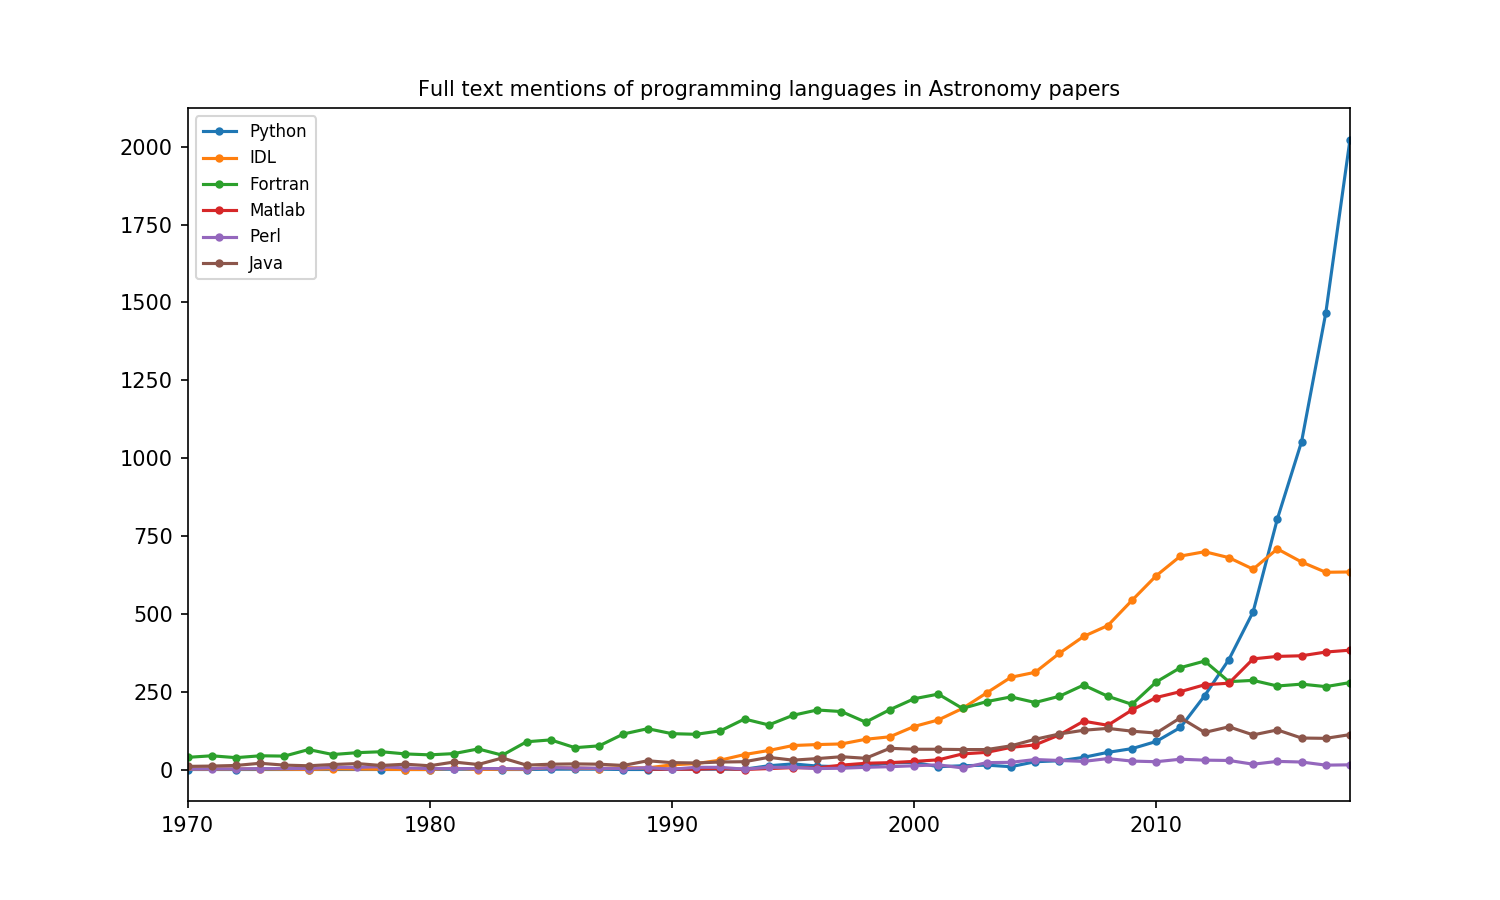
\includegraphics[width=0.7\textwidth]{python-astro-citations.png}
  \caption{Mentions of programming languages in refereed Astronomy papers}\label{fig:python-astro-citations}
\end{figure}

Deliverable: \localdelivref{application-astro}

\TODO{HF: The deliverable should either be a software (OTHER) or a
  demonstrator (DEM), I think. A report will be required in addition
  in either case through the deliverable reporting.}

\TODO{Should Quantstack be a partner here? They are the widget
  experts.}


\end{task}
